\section{Wahrscheinlichkeitstheorie}
%\renewcommand{\baselinestretch}{1.25}\normalsize
	\subsection{Kombinatorik}
		\begin{minipage}{13.5cm}
		\begin{tabular}{| p{5.5cm} | c | c |}
			\hline
			Art der Auswahl bzw. Zusammenstellung von $k$ aus $n$ Elementen	& \multicolumn{2}{c|}{Anzahl der Möglichkeiten}\\
 			& ohne Wiederholungen		& mit Wiederholungen\\
 			& $(k\leq n)$ 				& $(k\leq n)$ \\
 			\hline
 			Permutationen & $P_n=n!(n=k)$ &
 			$P_n^{(k)}=\frac{n!}{k!}$ \\ & &\\
 			Kombinationen & $C_n^{(k)}=\binom n k$ &
 			$C_n^{(k)}=\binom{n+k-1} k$\\
 			& &\\
 			Variationen & $V_n^{(k)}=k!\binom n k$ & $V_n^{(k)}=n^k$\\
 			\hline
		\end{tabular}
		\end{minipage}
		\begin{minipage}{5cm}
		$\binom n k$ mit TR: \texttt{nCr(n,k)} \hspace{9.3mm}En\\
		\hspace*{19mm} \texttt{Kombinat(n,k)} De
		\end{minipage}
		\begin{list}{$\bullet$}{\setlength{\itemsep}{0cm} \setlength{\parsep}{0cm} \setlength{\topsep}{0.1cm}} 
         	\item \textbf{Permutationen}: Gegeben seien $n$ verschiedene Objekte. Dann gibt es $n!$
         	verschiedene Reihenfolgen in denen man diese Objekte anordnen
         	kann. \\
         	z.B.: $x,y,z;\quad x,z,y;\quad z,y,x;\ldots$
         % \item Permutation nennt man eine Anordnung von $n$ Elementen in einer Bestimmten
		%		Reihenfolge
		 	\item \textbf{Kombination}: Gegeben seien $n$ verschiedene Objekte. Dann gibt es $\binom n k$
		 	Möglichkeiten, daraus $k$ Objekte auszuwählen, wenn es nicht auf die Reihenfolge
		 	ankommt. \\
		 	z.B.: Wie viele verschiedene Möglichkeiten hat man beim Lotto, 6 Zahlen aus 49
		 	auszuwählen?
		 % \item Kombination nennt man eine Auswahl von $k$ Elementen aus $n$ Elementen
		 % 		ohne Beachtung der Reihenfolge
		  \item \textbf{Variation} nennt man eine Auswahl von $k$ Elementen aus $n$
		  		verschiedenen Elementen unter Beachtung der Reihenfolge
        \end{list}
        

\vspace{5mm}
	\begin{minipage}{6.8cm}
	\subsection{Wahrscheinlichkeit}
		\begin{tabular}{ll}
			Wertebereich:
			& ${0}\le{P(A)}\le{1}$\\ \\
			Sicheres Ereignis:
			& $P(\Omega)=1$\\ \\
			unmögliches Ereignis:
			& $P(\emptyset)=0$
		\end{tabular}
	\end{minipage}
		\begin{minipage}{11.2cm}
		\textbf{Rechenregeln}\\
			\begin{tabular}{ll}
				komplementär Ereignis:
				&$P(\bar{A})=P({\Omega}\setminus{A})=1-P(A)$\\ \\
				Differenz der Ereignisse A und B:
				&$P({A}\setminus{B})=P(A)-P({A}\cap{B})$\\ \\
				Vereinigung zweier Ereignisse:
				&$P({A}\cup{B})=P(A)+P(B)-P({A}\cap{B})$
			\end{tabular}
		\end{minipage}
\vspace{1mm}

	
	\subsection{Laplace-Ereignisse  }
    	In einem endlichen Wahrscheinlichkeitsraum $\Omega$ haben alle
    	Elementarereignisse die gleiche Wahrscheinlichkeit.
    	\begin{center}
    	$P(A)=\dfrac{\left| A\right|}{\left|\Omega\right|}$
    	\end{center}

	\subsection{Unabhängige Ereignise  }
		Unabhängige Ereignisse $A$ und $B$ liegen vor, wenn:\\
    	\hspace*{8mm} $P(A\mid B)=P(A)$ \hspace{4mm} und \hspace{4mm}
    	$P(B\mid A)=P(B)$\\
    	erfüllt ist. Für sie gilt\\
    	\hspace*{8mm} $P(A\cap B)=P(A)P(B)$\\
    	Die Tatsache, dass A eingetreten ist, hat keinen Einfluss auf die 
		Wahrscheinlichkeit von B.\vspace{1mm}



	\subsection{Bedingte Wahrscheinlichkeit  }
		Die Wahrscheinlichkeit für das Eintreten des Ereignisses $A$ unter der
		Bedingung, dass das Ereignis $B$ bereits eingetreten ist.
		\begin{center}
		$P(A\mid B)= \dfrac{P(A\cap B)}{P(B)}=\underbrace{\frac{P(A)\cdot
		P(B)}{P(B)}=P(A)}_{\text{nur wenn unabhängig}}$ 
		\end{center}



	\subsection{Satz von Bayes  }
		\begin{tabular}{ll}
		$P(B\mid A)=P(A\mid B) \cdot\dfrac{P(B)}{P(A)}$\vspace{1mm}
		\end{tabular}


	\subsection{Totale Wahrscheinlichkeit  }
		\begin{tabular}{ll}
        $P(A)=\sum\limits_{i=1}^N P(A\mid G_i)\cdot P(G_i)$
        \end{tabular}

	
\subsection{Wahrscheinlichkeitsverteilung}

	\subsubsection{Verteilungsfunktion}
		\renewcommand{\arraystretch}{1.5}
		\begin{tabular}[]{|l|l|}
        	\hline
        	\textbf{diskret} & \textbf{kontinuierlich}\\
        	\hline
        	\hline
        	$P(X\leq x)=F(x)=\sum\limits_{k=-\infty}^x p_k$ &
        	$P(X\leq x)=F(x)=\int\limits_{-\infty}^x\varphi(\tilde{x})d\tilde{x}$\\
  			$P(X>x)=1-P(X\leq x)$ & 
  			$P(X>x)=1-P(X\leq x)$\\     
  			   
        	$P(\alpha_1 \le X \leq \alpha_2)=F(\alpha_2)-F(\alpha_1)=\sum\limits_{k=\alpha_1}^{\alpha_2} p_k$ &        	
  			$P(\alpha_1 \le X \leq \alpha_2)=F(\alpha_2)-F(\alpha_1)=\int \limits_{\alpha_1}^{\alpha_2}\varphi(\tilde{x})d\tilde{x}$\\
  		
  			$F_{x_1,x_2}(\alpha_1,\alpha_2)=P(\alpha_1 \le X_1 , \alpha_2\leq X_2)$&
  			$F_{x_1,x_2}(\alpha_1,\alpha_2)=P(\alpha_1 \le X_1 , \alpha_2\leq X_2)$\\
          	\hline
        \end{tabular}
		\renewcommand{\arraystretch}{1}

		\textbf{Eigenschaften}
  				$$\boxed{\mathbb{D}(F) = \mathbb{R}} \qquad \boxed{\mathbb{W}(F)
  				\in[0,1]} \qquad \boxed{F(-\infty)=0} \qquad  \boxed{F(\infty)=1}
  				\qquad \boxed{F(x) \text{ ist monoton steigend}}$$


	\subsubsection{Wahrscheinlichkeitsdichte }
		\begin{tabular}{p{7.3cm}p{8.5cm}}
    	$\varphi(x)=F'(x)$ &Dichtefunktion oder Wahrscheinlichkeitsdichte\\
    	$\varphi_{x_1,x_2}(\alpha_1,\alpha_2)=\frac{\delta^2}{\delta_{x_1}\delta{x_2}}F_{x_1,x_2}(\alpha_1,\alpha_2)$ &Dichtefunktion oder Wahrscheinlichkeitsdichte mit mehreren Variablen\\
    	
    	\multirow{2}{11cm}{Bei Sprungstellen von F(x): }\\
    	\multirow{2}{11cm}{$\varphi(x) = $ Dirac mit Gewichtung der Sprunghöhe}
    	\end{tabular}


	\subsubsection{Rechenregeln für $\varphi$ und $F$ }
		\begin{minipage}{11cm}
			\begin{tabular}{ll}
        	Gegeben: &X, Y Zufallsvariablen\\
        	&$\varphi_x$, $\varphi_y$ bekannt\\
        	\end{tabular}
 
        	\begin{tabular}{p{6cm}p{6cm}}
        	Verteilungsfunktion: &Dichte:\\
        	$F_{x+a}(x)=F_x(x-a)$  &$\varphi_{x+a}(x)=\varphi_x(x-a)$\\
        	$F_{\lambda x}(x)=F_x(\frac{x}{\lambda})$ &$\varphi_{\lambda
        	x}(x)=\varphi_x(\frac{x}{\lambda})\frac{1}{\lambda}$\\
        	$F_{x+y}(x)=F_x\ast\varphi_y(y)=F_y\ast\varphi_x(x)$ &
        	$\varphi_{x+y}(x)=\varphi_x\ast\varphi_y(x)$\\
        	$F_{\sqrt{x}}(x)=F_x(x^2)$ &
        	$\varphi_{\sqrt{x}}(x)=2x\varphi_x(x^2)$\\
        	$F_{x^2}(x)=F_x(\sqrt{x})$ &
        	$\varphi_{x^2}(x)=\frac{1}{2}x^{-\frac{1}{2}}\varphi_x(\sqrt{x})$
        	\end{tabular}
		\end{minipage}
		\begin{minipage}{7cm}
        	\textbf{Algorithmus Bsp.}
        	\begin{tabular}{ll}
        	1. Definition von $F$ anwenden: $F_{\lambda x}(x)=P(\underbrace
        	{\lambda X\leq x}_{*})$\\ 
        	2. Bedingung * umformen: $P(X \leq
        	\frac{x}{\lambda})=F_x(\frac{x}{\lambda})$\\ 
        	3. für Dichte: $\frac{d}{dx}$\\
        	\vspace{3mm}
        	$\varphi_{\lambda x}(x)=\frac{d}{dx}F_{\lambda
        	x}(x)=\frac{d}{dx}F_x(\frac{x}{\lambda})=
        	\varphi_x(\frac{x}{\lambda})\frac{1}{\lambda}$
        	\end{tabular}
			\vspace{10mm}
        \end{minipage}

        
        
        
        \subsubsection{Erwartungswert}
		Sei $X$ eine Funktion auf $\Omega$, und lasse sich $\Omega$ in endlich viele
		Ereignisse, auf denen $X(\omega)$ konstant ist, $A_i$ zerlegen, dann ist der
		Erwartungswert von $X$\\
        $Erwartungswert = \sum Wert \cdot Wahrscheinlichkeit$\\
		$E(X)=\sum\limits_{i=0}^n \underbrace{a_i}_{\text{Wert}}\cdot \underbrace{P(X=a_i)}_{\text{W'keit}}=\int\limits_{-\infty}^\infty \alpha \cdot \varphi_x(x)d\alpha$\\
		$E(y)=E(g(x))=\int\limits_{-\infty}^\infty g(\alpha) \cdot \varphi_x(x)d\alpha$ \hspace{2mm} für $y=g(x)$\\
		

		\textbf{Rechenregeln}\\
			\begin{tabular}{ll}
    		$E(X+Y)=E(X)+E(Y)$\\
    		$E(\lambda X + \mu)=\lambda \cdot E(X) + \mu$ & $\lambda, \mu \in \mathbb{R}$\\
    		$E(XY) = E(X)\cdot E(Y)$ & wenn X,Y unabhängig sind\\
    		\end{tabular}
      
	\subsubsection{Varianz }

		\begin{tabular}{ll}
		$var(x)=\sigma ^2=E[(X-E(X))^2]=E(X^2)-E(X)^2$\\$=\int\limits_\infty^\infty(\alpha - E(x))^2\varphi_x(\alpha)d\alpha$\\
		\end{tabular}
		
		\textbf{Rechenregeln}\\
			\begin{tabular}{ll}
        	$var(\lambda X)=\lambda^2 var(X) \qquad $ $\lambda, \mu \in
        	\mathbb{R}$\\ 
        	$var(X_1+X_2+\ldots+X_n) \neq var(n X)$ \\
        	$var(X+Y)= \begin{cases}
	                      var(X)+var(Y)
	                      &	\text{(X,Y unabh.)}\\                     
	                      var(X) + var(Y) + 2 \cdot cov(X,Y) 
	                      &	\text{(X,Y abhängig)}\\
                     \end{cases} $ \\
        	$var(X Y)= var(Y)var(X)+var(Y)E(X)^2+var(X)E(Y)^2$
        	\end{tabular}
        	
		\subsubsection{Korrelation / Correlation}
		\begin{tabular}{ll}
        $r_{xy}=E(XY^*)$
        \end{tabular}
		\subsubsection{Kovarianz / Covariance}
		\begin{tabular}{ll}
        $c_{xy}=cov(X,Y)=E((x-E(X))(y-E(Y)))$\\$=E(XY^*)-E(X)E(Y)=\underbrace{0}_{\text{falls X,Y unabhängig}}=
        \underbrace{r_{xy}}_{\text{falls X,Y mittelwertsfrei}}$
        \end{tabular}
        \subsubsection{Korrelations Koeffizient / Correlation Coefficient}
		$\rho_{xy}=\frac{E((X-m_x)\cdot(Y-m_y)^*)}{\rho_x \rho_y}$\\
		$|\rho_{xy}\leq 1|$ \\ 
		\textbf{Unabhängig}\\
		Zwei Zufallsvariablen sind statitisch unabhängig wenn die Wahrscheindlichkeitsdichtefunktion separierbar ist: \\
		$\varphi_{xy}(\alpha, \beta) = \varphi_x(\alpha)\varphi_y(\beta) \Longrightarrow$ auch $E(XY)=E(X)E(Y)$ \\
		Wenn die Variablen zusätzlich unkorreliert sind zählt: $Var(X+Y) = Var(X) + Var(Y)$
		
		
		
	\subsubsection{Momenterzeugende Funktion - moment generating function}
		Die momenterzeugende Funktion ist eine Darstellung aller Momente einer Verteilung. 
		$\Phi(t)=E(e^{tX})=\int\limits_{-\infty}^\infty e^{tx} \cdot \varphi(x) dx$ bzw. $= \sum\limits_{i=1}^{\infty}e^{tx_i} \cdot P(X=x_i)$	\\
		$\Phi(t)$ heisst Momenterzeugende Funktion weil: \\
		$\frac{d^n}{dt^n}\Phi(t)=)=\int\limits_{-\infty}^\infty x^n \cdot e^{tx} \cdot \varphi(x) dx$ bzw. $= \sum\limits_{i=1}^{\infty} x_i^n \cdot e^{tx_i} \cdot P(X=x_i)$\\
		für $\frac{d^n}{dt^n}\Phi(0)=)=\int\limits_{-\infty}^\infty x^n \cdot \varphi(x) dx$ bzw. $= \sum\limits_{i=1}^{\infty} x_i^n \cdot P(X=x_i) = E(X^n)=\mu_n $\\
		
		Falls $\Phi_x(t) = \Phi_y(t)$ dann gilt auch $F_x(x)=F_y(x)$. Dass heisst eine Wahrscheinlichkeitsverteilung kann eindeutig zu einer momenterzeugende Funktion zugeordnet werden.
		
		
			
	\subsubsection{Verschiedene Wahrschenlichkeitsdichtenfunktionen}
		\textbf{Gauss Verteilung/ Normal Distribution}\\
 		\begin{minipage}{10cm}
		Viele kleine, unabhängige Zufallsvariable sammeln sich zu einer
		normalverteilten Zufallsvariable.\\
		 $\varphi(x)=\frac{1}{\sqrt{2
		\pi}\sigma}\cdot e^{-\frac{(x-\mu)^2}{2\sigma^2}} = N(\mu ; \sigma^2) $\\ 
		$F(x)=\frac{1}{\sqrt{2
		\pi}\sigma}\cdot \int\limits^{x}_{-\infty}{e^{-\frac{(\tilde{x} -\mu)^2}{2\sigma^2}}} $ \\
		\textbf{Standardisierung}\\
		Erwartungswert: $E(X)=\mu$ \hspace{4mm}(=0 bei Standardnormalver.)\\ 
		Varianz \hspace{11.5mm}: $var(X)=\sigma^2$ (=1 bei Standardnormalver.)\\ \\
		$x=\dfrac{X-\mu}{\sigma}$ \hspace{5mm} $x$ aus Tabelle
		\end{minipage}
		\hspace{5mm}
		\begin{minipage}{7.5cm}
		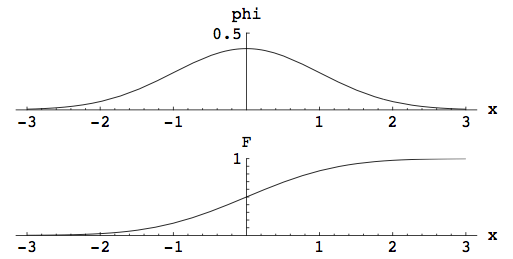
\includegraphics[width=7.5cm]{bilder/normalverteilung.png}
		Dichtefunktion (oben) und Verteilungsfunktion (unten) der Normalverteilung. 
   		\end{minipage} \\ \\
		$ 68\% $ der Werte liegen im Intervall $[ \mu - \sigma, \mu + \sigma]$, 
		$95\% $ in $[ \mu - 2\sigma, \mu + 2\sigma]$, 	
		$99.7\% $ in $[ \mu - 3\sigma, \mu + 3\sigma]$\\\\
		\textbf{ Normalverteilung mit mehreren Unbekannten}\\
		$\varphi_{x,y}(\alpha,\beta)=\frac{1}{2\pi \sigma_x \sigma_y \sqrt{1-\rho_{xy}^2}}
			e^{-\frac{1}{2(1-\rho_{xy})^2} + \frac{(\alpha - m_x)^2}{\sigma_x^2} 
			- 2\rho_{xy}\frac{(\alpha - m_x)\beta - m_y)^2}{\sigma_x \sigma_y} + \frac{(\beta - m_y)^2}{\sigma_y^2}}$\\
			$\varphi_x(\textbf{x})=\frac{1}{(2\pi)^{\frac{n}{2}}|\textbf{C}_x|^{\frac{1}{2}}}\cdot 
			e^{-\frac{1}{2}(\textbf{x} - \textbf{m}_x)^T \textbf{C}_x^{-1} (\textbf{x} - \textbf{m}_x)}$ mit \\
			$\textbf{m}_x=[E(x_1), E(x_2), \ldots, E(x_n)]^T$ und der Kovarianzmatrixe $\textbf{C}_x$; $c_{ij} = E((x_i-E(x_i)(x_j-E(x_j))))$ \\
		\textbf{Rechenregel für die Normalverteilung mit mehreren Unbekannten}
		\begin{itemize}
		  \item wenn $z=a x + b y$ dann ist \\
		  $m_z =  a m_x + b m_y$\\
		  $\sigma_z^2 = a^2\sigma_x^2 + b^2\sigma_y^2+2ab\sigma_x\sigma_y$
		  \item wenn x und y unkorreliert sind, dann ist \\
		  		$f_{x,y}(\alpha, \beta) = \varphi_x(\alpha)\varphi_y(\beta)$ dass heisst x und y sind auch statistisch unabhängig.
		  \item Der optimale nicht lineare Schätzer für die Werte $\mu$ und $\sigma$ ist gleich dem lineare Schätzer.
		\end{itemize}
   		
 
        
        
        
\subsection{Zufallsprozesse}
\begin{minipage}{10.3cm}
	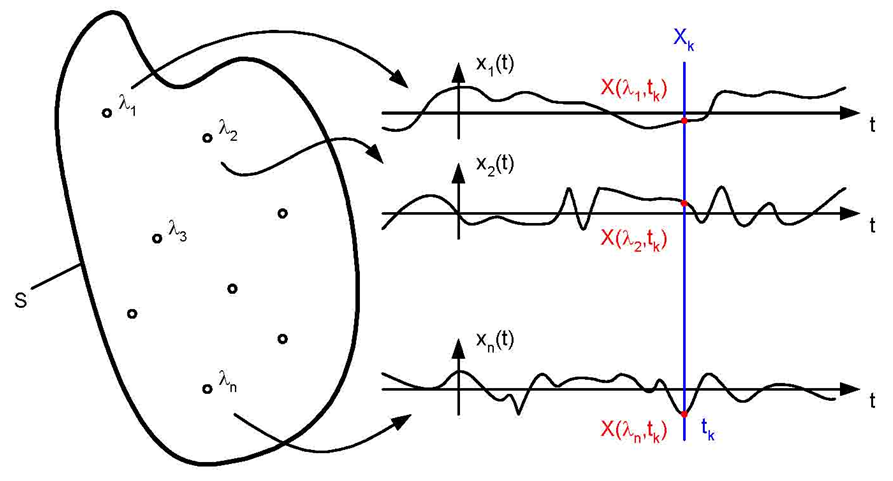
\includegraphics[width=10cm]{bilder/zufallsprozess.png}
\end{minipage}
\begin{minipage}{8.5cm}
	Bei einem \textbf{Zufallsprozess} wird jedem \textbf{Ergebnis} \boldmath$\lambda$ aus 
	dem \textbf{Ergebnisraum} $S$ eine \textbf{deterministische} \textbf{Funktion} $x(\lambda, t)$
	\unboldmath zugewiesen. \\
	Zufallsprozesse beschreiben eine deterministische Zeitfunktion ausgelöst durch ein Ergebnis eines
	Zufallsexperiments. z.B $sin(\omega t + X)$ wobei X eine Zufallsvariable ist, welche zu Beginn aus dem Ereignisraum zugewiesen wird\\
	Zeitlich \textbf{zufällig ablaufende Funktionen} können ebenfalls als \textbf{deterministische} Funktionen 
	\textbf{aufgefasst} werden, bei denen der Beobachter nie weiss, welche Funktion $x_\lambda(t)$ konkret
	vorliegt.	\\ \\
	Zum Vergleich: Bei Zufallsvariablen wird jedem Elementarereignis eine Zahl zugewiesen. 
\end{minipage} 
\vspace{0.5cm} \\

\subsubsection{Statistische Mittelwerte (Scharmittel)}
Die statistischen Mittelwerte sind eine Funktion der Zeit $t$, da es sich um Mittelwerte über das
Ensemble (ganzer Ergebnisraum) handelt. Hierbei werden alle deterministischen Funktionen zu einem
bestimmten Zeitpunkt $t$ gemittelt. 

\renewcommand{\arraystretch}{1.4}
\begin{tabular}[c]{ p{4.5cm}  p{13.5 cm}  }
	\textbf{Erwartungswert}: 	&  $\mu_{x}(t) = E\left[X(t)\right] =
          \int\limits_{-\infty}^{+\infty} x \cdot f_{x}(x;t)\;dx$ bzw $=\frac{1}{N}\sum\limits_{i=1}^{N}x_i(n)$ \\
    \textbf{Erwartungswert eines deterministischen Signals}:& $\mu_f(t) = E(f(t))=f(t)$\\
 	\textbf{Varianz}: &         $\sigma_x^2(t)=E((x(t)-\mu_x(t))^2)=c_x(t_1,t_1)$
    
	 
\end{tabular}
\renewcommand{\arraystretch}{1}


\subsubsection{Stationarität}
Ein stationärer Prozess verändert seine statistischen Eigenschaften über die Zeit nicht. \\

\textbf{Streng Stationär (SSS - Strict Sense Stationary)}\\
% TODO genaue beschreibung streng, schwach stationär
Bei einem streng stationären Prozess bleiben die n-dimensionale WSK-Dichten über die
Zeit konstant. D.h. die \textbf{statistischen Eigenschaften} und somit auch die WSK-Dichten sind zu 
\textbf{allen Zeitpunkten dieselben}.
$$ f_x(x_1, x_2, \ldots, x_n; t_1, t_2, \ldots, t_n) =
		f_x(x_1, x_2, \ldots, x_n; t_1+c, t_2+c, \ldots, t_n+c) \qquad \forall (c,n \in
		\mathbb{R})$$
% Es gelten folgende Beziehungen: \\
% $$E[X(t)] = \mu_{x} \qquad \qquad
% r_{xx}(t_{1},t_{2}) = r_{x}(\tau),\quad \text{ mit } \tau = t_{2} - t_{1} \qquad \qquad
% c_{xx}(t_{1},t_{2}) = r_{x}(\tau) - \mu_{c}^{2}$$ 

\textbf{Schwach Stationär (WSS - Wide Sense Stationary) - Stationarität 2. Ordnung}\\
Bei einem schwach stationären Prozess sind die statistischen Eigenschaften zwar
\textbf{nicht zu jedem Zeitpunkt die selben}, jedoch sind sie \textbf{nicht} von einem \textbf{absoluten} Zeitpunkt, sondern
von der \textbf{Differenz} ($\tau$) \textbf{zweier Zeitpunkte} ($t_1, t_2$) abhängig.  \\ 
$$ f_x(x_1, x_2; t_1, t_2) = f_x(x_1, x_2; t_1+c, t_2+c) \qquad \forall (c \in
		\mathbb{R})$$
%Zudem gilt:\\
\renewcommand{\arraystretch}{1.4}
\begin{tabular}[c]{ p{3.3cm}  p{6.5cm} p{8cm} }
	\textbf{Mittelwert}: 	&  $E[X(t)] = \mu_{x} = \text{const.}$  
							& bleibt über die ganze Zeit konstant\\ 
	\textbf{quad. Mittelwert}: 	&  $E[X^{2}(t)] = r_{x}(0)$  \\ 
	\textbf{Autokorrelation}: 	& 	$r_{xx}(t_{1},t_{2}) = r_{x}(\tau)$
	& \multirow{2}{8cm}{nur \textbf{abhängig} von der \textbf{Zeitdifferenz} $(\tau = t_2 - t_1)$ und \textbf{nicht direkt} von
	 der \textbf{Zeit} $t$} \\
	 \textbf{Autokovarianz}:		& $ c_{xx}(t_{1},t_{2}) = r_{x}(\tau) - \mu_{x}^{2} = c_{xx}(\tau)$ \\
\end{tabular}
\renewcommand{\arraystretch}{1}
 
Bei einem Zufallsprozess handelt es sich immer um ein WSS-Prozess, sobald der Erwartungswert
konstant ist und die Autokorrelationsfunktion nur eine Funktion von $\tau$ ist, d.h. beide 
statistischen Kennwerte bzgl. einer zeitlichen Verschiebung unabhängig sind.    
Jeder streng stationäre Prozess ist auch schwach stationär, aber nicht umgekehrt. 
        
%   \item Zwei Zufallsprozesse heissen Verbund-schwach-station\"ar, wenn jeder Prozess f\"ur sich 
%         schwach-station\"ar ist und zudem gilt:  
%         \begin{itemize}
%           \item[$\circ$] $r_{xy}(t_{1},t+\tau) = E[X(t)Y(t+\tau)] = r_{xy}(\tau)$ 
%         \end{itemize} 
%   \item Dann gilt auch:
%   \begin{itemize}
%      \item[$\circ$] $c_{xy}(\tau) = r_{xy}(\tau) - \mu_{x} \mu_{y}$
%   \end{itemize} 
% \end{itemize} 

%TODO verbund schwach stationär

\subsubsection{Zeitliche Mittelwerte (Zeitmittel)}
Hierbei werden die jeweiligen deterministischen Funktionen (Musterfunktionen) zeitlich gemittelt.
Wird das zeitliche Mittel über den gesamten Zufallsprozess berechnet, so handelt es sich bei den
zeitlichen Mittelwerten um \textbf{Zufallsvariablen}, d.h. die folgenden zwei Ausdrücke sind
abhängig davon (darum Index $_i$), welche Funktion genutzt wird.

%\renewcommand{\arraystretch}{1.4}
\begin{tabular}[c]{ p{4cm}  p{14.5cm}  }
	\textbf{Mittelwert}: 	&  
	$\overline{x_{i}} = \left\langle x_{i}(t) \right\rangle = 
           \lim\limits_{T \rightarrow \infty}
             \frac{1}{T} \int\limits_{-\frac{T}{2}}^{+\frac{T}{2}} x_{i}(t) \; dt$ \\
   	\textbf{Autokorrelation}: 	& 	
   	$\overline{r}_{x_{i}x_{i}}(\tau) = \left\langle x_{i}(t) \cdot x_{i}(t+\tau) \right\rangle = 
           \lim\limits_{T \rightarrow \infty}
             \frac{1}{T} \int\limits_{-\frac{T}{2}}^{+\frac{T}{2}} x_{i}(t) \cdot x_{i}(t + \tau) \; dt$\\
    \multicolumn{2}{l}{Falls der \textbf{Prozess stationär} ist gilt zudem: } \\
	\textbf{Mittelwert}: 	&  
	$E[\overline{x}] = 
           \lim\limits_{T \rightarrow \infty}
             \frac{1}{T} \int\limits_{-\frac{T}{2}}^{+\frac{T}{2}} E[x(t)] \; dt = 
             \frac{1}{T} \int\limits_{-\frac{T}{2}}^{+\frac{T}{2}} \mu_{x} \; dt = \mu_{x}$  \\
   	\textbf{Autokorrelation}: 	& 	
   	$E[\overline{r}_{xx}(\tau)] = 
           \lim\limits_{T \rightarrow \infty}
             \frac{1}{T} \int\limits_{-\frac{T}{2}}^{+\frac{T}{2}} E[x(t)x(t+\tau)] \; dt =
             \frac{1}{T} \int\limits_{-\frac{T}{2}}^{+\frac{T}{2}} r_{xx}(\tau) \; dt = r_{xx}(\tau)$\\
\end{tabular}
\renewcommand{\arraystretch}{1}

\subsubsection{Ergodizität}
Ein stationärer Prozess ist zudem noch ergodisch, wenn die \textbf{zeitlichen Mittelwerten} den
\textbf{statistischen Mittelwerten entsprechen}. %\hspace{2cm} \textbf{Zeitmittel = Scharmittel}\\ 


	\begin{minipage}{5cm}
		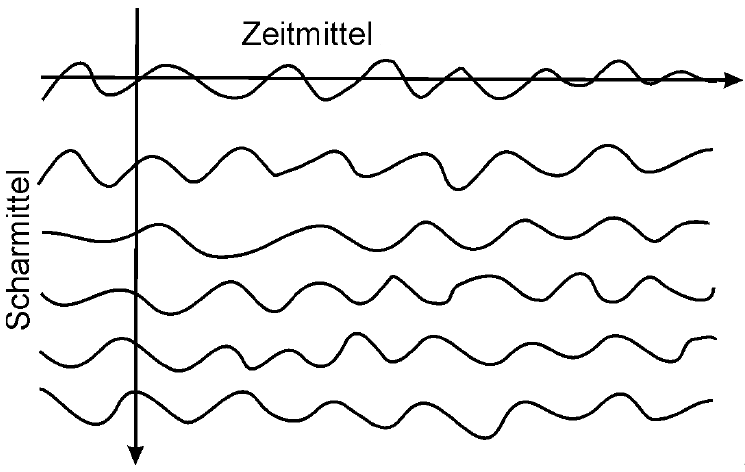
\includegraphics[width=4.5cm]{bilder/zeit-scharmittel.png}
  	\end{minipage}
	\begin{minipage}{13.5cm}

	\begin{tabular}{ll}
  		\multicolumn{2}{l}{Nur bei ergodischen Prozessen gilt zwingend:} \\ \\
      $E[X(t)] = \overline{x} = \left\langle x(t) \right\rangle$ & DC-Level \\
      $E[X(t)]^{2} = (\overline{x})^{2} = \left\langle x(t) \right\rangle^{2}$ & DC-Leistung \\
      $E[X^{2}(t)] = r_{xx}(0) = \overline{x^{2}} = 
                     \left\langle x^{2}(t) \right\rangle $ & Gesamtleistung \\
      $\sigma_{x}^{2}(t) = \left\langle x^{2}(t) \right\rangle 
                           - \left\langle x(t) \right\rangle^{2}$ & AC-Leistung \\
      $\sigma_{x}(t) = \overline{\sigma}_{x}$ & RMS-Level (Effektivwert) des AC-Signals\\
    \end{tabular} \\
  	\end{minipage}


\subsubsection{Vergleich Stationär - Ergodisch}
\textbf{Mückenschwarm:}\\
\textbf{Ergodisch:} Fliegen alle Mücken zusammen in einem Schwarm, so fliegt jede Mücke über die
ganze Zeit gemittelt (Zeitmittel) so schnell wie der ganze Schwarm im Mitel (Scharmittel), ansonsten
würde der Schwarm nicht zusammenhalten können. \\
\textbf{Stationär:} Ist eine Mücke krank und kann mit dem Schwarm nicht mithalten, so fliegt sie
alleine und v.a. langsamer. Somit ist ihre Durchschnittsgeschwindigkeit (Zeitmittel) nicht gleich
derjenigen des Schwarms (Scharmittel), also kommt sie später am Ziel an. \\
\textbf{Weder noch:} Fliegen die Mücken nach dem Start immer langsamer, so ist die
durchschnittliche Geschwindigkeit des Schwarms (Scharmittel) nicht konstant.

\textbf{Schulnoten:}\\
\textbf{Ergodisch:} Alle Schüler müssten dieselbe Zeugnisnote (Zeitmittel) haben und zudem müsste
diese Note jeweils auch dem Klassenschnitt (Scharmittel) der einzelnen Prüfungen entsprechen. \\
\textbf{Stationär:} Der Klassenschnitt (Scharmittel) ist bei jeder Prüfung gleich, jedoch gibt es
unterschiedlich starke Schüler mit unterschiedlichen Zeugnisnoten (Zeitmittel). \\
\textbf{Weder noch:} Der Klassenschnitt (Scharmittel) ist immer unterschiedlich.

\textbf{Thermisches Widerstandsrauschen:} \\
Dies ist bei gleichbleibender Temperatur \textbf{ergodisch}.

\subsubsection{Korrelationen und Leistungsspektren}
Formeln in diesem Abschnitt gelten für \textbf{stationäre} Prozesse. \\

\renewcommand{\arraystretch}{1.6}
\begin{tabular}[c]{ p{3.5cm}  p{6cm} p{7.5cm} }
	\textbf{Autokorrelation}: 	&  
	\multicolumn{2}{l}{$r_x(t_1,t_2)=r_x(t_1-t_2)=r_x(\tau)=r_{xx}(\tau) = E[X(t)X(t+\tau)]$} \\
  	&	$\mid \! r_{xx}(\tau) \! \mid \leq r_{xx}(0) = E[X^{2}(t)]$ 
	& $r_{xx}(-\tau) = r_{xx}(\tau) \quad$ (gerade, Fouriertransformation wird real)\\
  \textbf{Kreuzkorrelation}:& 	
 	$r_{xy}(\tau)=r_{xy}(\tau) = E[X(t)Y(t+\tau)]$  
	& $r_{xy}(-\tau) = r_{yx}(\tau) \quad$ (Reihenfolge Indizes!) \\
    & $|r_{xy}(\tau)| \leq \frac{1}{2} \left[ r_{xx}(0)+r_{yy}(0)\right] $
	& $|r_{xy}(\tau)|  \leq \sqrt{r_{xx}(0)r_{yy}(0)}$ \\
   \textbf{Autokovarianz }: 	&  \multicolumn{2}{l}{$c_{xx}(t_{1},t_{2}) =
          E\left[ \left( X(t_{1})-\mu_{x}(t_{1})\right) \cdot
                  \left( X(t_{2})-\mu_{x}(t_{2})\right) \right] =
          r_{xx}(t_{1},t_{2}) - \mu_{x}(t_{1}) \cdot \mu_{x}(t_{2})=$}\\	
	&\multicolumn{2}{l}{$c_x(\tau)=c_{xx}(\tau) = E\!\left[ \left( X(t)      - E[X(t)]      \right) \cdot
                                  \left( X(t+\tau) - E[X(t+\tau)] \right) \right] =
                        r_{xx}(\tau) - \mu^{2}_{x} $} \\
   	\textbf{Kreuzkovarianz}: 	& \multicolumn{2}{l} {$c_{xy}(t_{1},t_{2}) = 
          E\left[ \left( X(t_{1})-\mu_{x}(t_{1})\right) \cdot
                  \left( Y(t_{2})-\mu_{y}(t_{2})\right)^* \right] =
          r_{xy}(t_{1},t_{2}) - \mu_{x}(t_{1}) \cdot \mu_{y}(t_{2})=$}\\	
   	&\multicolumn{2}{l}{$c_{xy}(\tau) = E\!\left[ \left( X(t)      - E[X(t)]      \right) \cdot
                                  \left( Y(t+\tau) - E[Y(t+\tau)] \right) \right] =
                        r_{xy}(\tau) - \mu_{x}\mu_{y} $}\\
    & \multicolumn{2}{l}{Zufallsprozesse bezeichnet man als zueinander
                        \textbf{unkorreliert}, wenn $c_{xy}(\tau) = 0$}
\end{tabular}
\renewcommand{\arraystretch}{1}

\textbf{Spektrale Leistung}\\
Autokorrelationsfunktion $r_{xx}(\tau)$ und Leistungsspektraldichte $P_{xx}(\omega)$ bilden ein
Fourier-\textbf{Transformationspaar}. \\ Die Leistungsspektraldichte kann als \textbf{mittlere Leistung pro Frequenzband }aufgefasst werden, sie ist
wie folgt definiert:                             
        $$ P_{xx}(\omega) = E\left[ \lim\limits_{T \rightarrow \infty}
                                    \frac{1}{T} \cdot \mid\! X(\omega) \!\mid^{2}\right]                          
                            = \int\limits_{-\infty}^{+\infty} r_{xx}(\tau) \cdot e^{-j\omega\tau} \; d\tau 
                            \qquad \IFT \qquad
        r_{xx}(\tau)   = \frac{1}{2\pi} \int\limits_{-\infty}^{+\infty} 
                             P_{xx}(\omega) \cdot e^{j\omega\tau} \; d\omega$$ 
        bzw:
         
        $$P_{xx}(z) = \sum\limits_{k=-\infty}^{\infty} r_{xx}(k)z^{-k}\qquad \IFT \qquad 
       	r_{xx}(k)=\frac 1{2\pi} \int \limits_{-\pi}^{\pi} P_{xx}(e^{jw})e^{jkw}dw \qquad 
       	r_{xx}(0) =\frac 1{2\pi} \int \limits_{-\pi}^{\pi} P_{xx}(e^{jw})dw = \lim\limits_{z \rightarrow 0} P_{xx}(z)$$
                             
$P_{xx}(\omega)$ ist rein reell, symetriesch $(P_{xx}(z)=P_{xx}^*(\frac{1}{z^*}))$ und $\geq 0$. \\
Kreuzkorrelationen ($r_{yx}(\tau), r_{xy}(\tau)$) und Kreuz-Spektraldichten ($P_{yx}(\tau),
P_{xy}(\tau)$) bilden ein Fourier-Transformationspaar.
\begin{center}
$ r_{yx}(\tau) \FT P_{yx}(\omega) \qquad \qquad r_{xy}(\tau) \FT P_{xy}(\omega)  $
\end{center}
Da die Autokorrelation sicher nicht kausal sind (auch für negative Zeitwerte definiert sind), muss die beidseitige z-Transformation angewendet werden.

Die Eigenwerte der Autokorrelationmatrix haben folgende Begrenzung:\\
$$\min\limits_\omega P_{xx}(z)\leq \lambda_i \leq \max\limits_{\omega}P_{xx}(z)$$

\subsubsection{Beispiele Autokorrelation}
\begin{tabular}{|l|l|l|}
%     \hline
%         \multicolumn{2}{|l|}{\textbf{Beispiele Autokorrelation}} \\
    \hline
        Weisses Rauschen
        & $r_{xx} (n) = \frac {N_0}{2} \delta(n) \FT P_{xx}(z)= \frac {N_0}{2};\hspace{0.25cm}$ & alle z\\
    \hline
        Prozess erster Ordnung
        & $r_{xx} (n) = P_s \cdot a^{|n|} \FT P_{xx} (z) = P_s \cdot \frac {1-a^2}{(1-az^{-1})(1-az)}$ & für $a<|z| < \frac{1}{a}$\\
    \hline
        
        & $r_{xx} (n) = a^n(u(n) - u(n-N)) \FT P_{xx} (z) = \frac{1-a^Nz^{-N}}{1-az^{-1}}$ & für $|z| > 0$\\
    \hline
        
        & $r_{xx} (n) = a^n \cdot u(n) \FT P_{xx} (z) = \frac{1}{1-az^{-1}}$ & für $|z| > a$\\
    \hline
        
        & $r_{xx} (n) = -a^n \cdot u(-n-1) \FT P_{xx} (z) = \frac{1}{1-az^{-1}}$ & für $|z| < a$\\
    \hline
        Binäres Datensignal
        & $r_{xx} (0) = P_s = A_1^2p_1 + A_0^2 p_0 $ &\\
        &$r_{ss} (|n| < T) = $ linearer Übergang von $r_{ss}(0)$ zu $r_{ss} (|n| = T)$ &\\
        & $r_{xx} (|n| \geq T) = P_s = A_1^2p_1^2 + A_0A_1p_0p_1 + A_1A_0p_1p_0 + A_0^2p_0^2$ &  \\
    \hline
        überlagerte Signale
        & $r_{gg\pm}(n) = r_{ss}(n) + r_{sf}(n) + r_{sf}(-n) + r_{ff}(n) $ &\\
        $g_\pm(t) = s(t) \pm f(t)$
        &  $\FT P_{g+}(\omega) = P_{s}(\omega) + P_{f}(\omega) \pm 2 \text{Re} \{P_{sf}(\omega) \}$ &\\ 
    \hline
\end{tabular} 
\vspace{-0.5cm}
\subsubsection{Numerische Berechnung}
\begin{tabular}{|l|l|}
    \hline
		\multicolumn{2}{|l|}{\textbf{Numerische Berechnung}} \\
    \hline
    Autokorrelation
        & $\hat{r}_{xx} (n) = \frac 1 N \sum\limits_{m=0}^{N-1} s(m ) s[(m+n) ] 
                                     = \frac 1 N \sum\limits_{m=0}^{N-1} s[(m-n) ] s(m ) \DFT \hat{P}_{xx}(z)$ \\
    \hline
    Kreuzkorrelation
        & $\hat{r}_{xy} (n ) = \frac 1 N \sum\limits_{m=0}^{N-1} s(m ) f[(m+n) ] 
                                     = \frac 1 N \sum\limits_{m=0}^{N-1} s[(m-n) ] f(m ) \DFT \hat{P}_{xy}(z) $ \\
    \hline
    Leistungsdichtespektrum 
        & $\hat{P}_{xx}(z) = \frac 1N \left|S_T(z)\right|^2 \IDFT \hat{r}_{xx} (n )
            \qquad \text{mit} \quad S_T(z) \IDFT s(n)$\\
    \hline
    Kreuz(leistungsdichte)spektrum 
        & $\hat{P}_{xy}(z) = \frac 1N S_T^*(z) F_T(z) \IDFT \hat{r}_{xy} (n )
        \qquad \text{mit} \quad F_T(z) \IDFT f(n)$\\
				
    \hline
\end{tabular}
\subsubsection{Übertragung von Zufallsprozessen durch LTI-Systeme}
Ein Zufallsprozess wird durch ein LTI-System übertragen. \hspace{2cm} $Y(t) = L[X(t)] \Rightarrow
Y(t) = h(t) \ast X(t)$ \vspace{0.3cm}\\
\renewcommand{\arraystretch}{1.4}
 \begin{tabular}[c]{ p{2cm}  p{8.5cm} p{8cm} }
	& \textbf{Allgemein} & \textbf{WSS-Prozess} \\
	\textbf{Mittelwert}
		& $\mu_{y}(t) = h(t) \ast \mu_{x}(t)$
		& $\mu_{y} = H(0) \mu_{x}$ \\
	\textbf{Auto-korrelation\textcolor{red}{*}}
		& {$r_{yy}(t_{1},t_{2}) = \int\limits_{-\infty}^{+\infty}
		\int\limits_{-\infty}^{+\infty} h(\alpha) h(\beta)
                      r_{xx}(t_{1}-\alpha, t_{2}-\beta) \; d\alpha \; d\beta$}
		& {$r_{yy}(\tau) = \int\limits_{-\infty}^{+\infty}
		\int\limits_{-\infty}^{+\infty} h(\alpha) h(\beta)
                      r_{xx}(\tau+\alpha-\beta) \; d\alpha \; d\beta$} \\
	\textbf{Spektrale Leistung}
		&
		& $P_{yy}(\omega)= H^{\ast}(\omega) H(\omega) P_{xx}(\omega)
			= |H(\omega)|^{2} P_{xx}(\omega)$  \\
\end{tabular}
\renewcommand{\arraystretch}{1} \\
\textcolor{red}{*} = Es ist viel einfacher die Autokorrelation aus der Spektralen Leistung
(Transformationspaar) - anstatt aus diesem höllischen Integral - auszurechnen. \\
Ein WSS-Prozess am Eingang erzeugt auch einen WSS-Prozess am Ausgang.

\subsubsection{Filterung von Zufallsprozessen}
Die Ausgangs Autokorrelation $r_y(k)$ ist\\
 $r_y(k) = r_x(k)\ast h(k) \ast h^*(-k)$ bzw. $\boxed{P_{y}(z) = P_{x}(z)\cdot H(z) \cdot H^*(\frac{1}{z^*}) \quad
  P_{y}(e^{j\omega})=P_x(e^{j\omega})\cdot|H(e^{j\omega})|^2}$

\subsubsection{Weisses Rauschen}
\begin{center}
	\begin{minipage}{8cm}
		$P_{xx}(\omega) = \dfrac{\eta}{2} \qquad r_{xx}(\tau) = \dfrac{\eta}{2} \cdot \delta(\tau)= \sigma_x^2 \cdot \delta(\tau)$ \\ \\
		Beispiel: therm. Rauschen von Widerständen \\
		\textbf{Nimmt} in der Praxis im \textbf{Tera-Hz Bereich ab}!
  	\end{minipage}
	\begin{minipage}{10cm}
		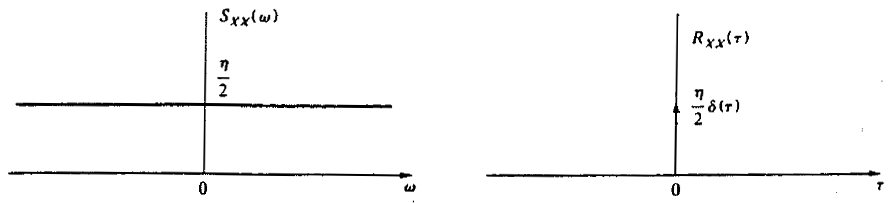
\includegraphics[width=9cm]{bilder/weisses_rauschen.png}
  	\end{minipage}
\end{center}

\subsubsection{Farbige Rauschsignale}
\renewcommand{\arraystretch}{2}
\begin{tabular}[c]{ | p{4cm} | p{3.5cm} | p{3cm} | p{6cm} | }
% 	\hline
% 		Weisses Rauschen
% 		& White Noise
% 		& $P_{xx}(\omega) = \dfrac{\eta}{2}$
% 		& \\
	\hline
		\textbf{Bezeichnung (De)}
		& \textbf{Bezeichnung (En)}
		& \textbf{Leist.-Spektrum}
		& \textbf{Anmerkung} \\
	\hline
		Rosa Rauschen
		& Pink Noise
		& $P_{xx}(\omega) = c \cdot \dfrac{1}{\omega}$
		& Testsignal für Tontechnik, wegen konstanter Leistung pro Oktave \\
	\hline
		Braunes/Rotes Rauschen
		& Brown/Red Noise
		&	$P_{xx}(\omega) = c \cdot \dfrac{1}{\omega^2}$
		& \\
	\hline
		Blaues Rauschen
		& Blue Noise
		&	$P_{xx}(\omega) = c \cdot \omega$
		& \\
	\hline
		Violettes Rauschen
		& Purple/Violet Noise
		&	$P_{xx}(\omega) = c \cdot \omega^2$
		& \\
    \hline
\end{tabular}
\renewcommand{\arraystretch}{1}

\subsection{Estimation \hayes{72}}
  \subsubsection{Bias}
    The bias is the difference between the real value $\Theta$ and the estimate $\hat{\Theta}$: 
    $B = \Theta - E(\hat{\Theta}_N)$. When $B=0$, the estimator is \em unbiased\em. When the estimator
    is biased but the bias goes to zero as the number of observations $N$ goes to infinity, then
    the estimator is \em asymptotically unbiased \em ($\lim_{N \rightarrow \infty} E(\hat{\Theta}_N) = \Theta$). 
    If the bias stays $B \neq 0$, the estimator is \em biased\em.
    
  \subsubsection{Consistency}
    If $\lim_{N \rightarrow \infty} Var(\hat{\Theta}_N) = 0$, the estimator is consistent. 
    $\hat{\Theta}_N$ is said to \em converge to $\Theta$ with probability one\em. 
    Here, a \em consistent \em estimator if it is asymptotically unbiased and has a variance that
    goes to zero as $N$ goes to infinity.
     
